% !TEX root = ../thesis.tex
\chapter{Data models}
\label{chap:data_model}
\label{sec:data_model}
\begin{comment}
This chapter describes the data model used by our architecture. In particular analyze the formalisms that lead the user to reach his network topology.

\end{comment}



This section details the three data abstractions introduced in Section~\ref{sec:gen_arch}, which are  used by the architecture shown in Figure~\ref{fig:orchestrator} to deploy the network services on the physical infrastructure. 
Our data models are inspired by the NFV ETSI standard~\ref{chap:the_state_of_the_art}, which proposes a service model composed of ``\textit{functional blocks}'' connected together to flexibly realize a desired service.
In order to meet the objectives described in the introduction, we declined this abstract model in multiple flavors according to the variegated granularity and details needed in the different layers.
All those models are inspired by the objective of integrating this functional component description of network services and topology and the possibility to model also existing network topology and services.  


\section{Service graph}
\label{sec:service_graph}

The \textbf{service graph (SG)} is an high level representation of the service to be implemented on the network, and it includes both aspects related to the infrastructure (e.g., which network functions implement the service, how they are interconnected among each other) % connections among the network functions implementing the service) 
and to the configuration of these network functions (e.g., network layer information, policies, etc.).

%IVANO: commento di fulvio: il SG comprende sia aspetti di infrastruttura che di configurazione del servizio

\begin{figure}%[h]
	\centering
	% left bottom right top
	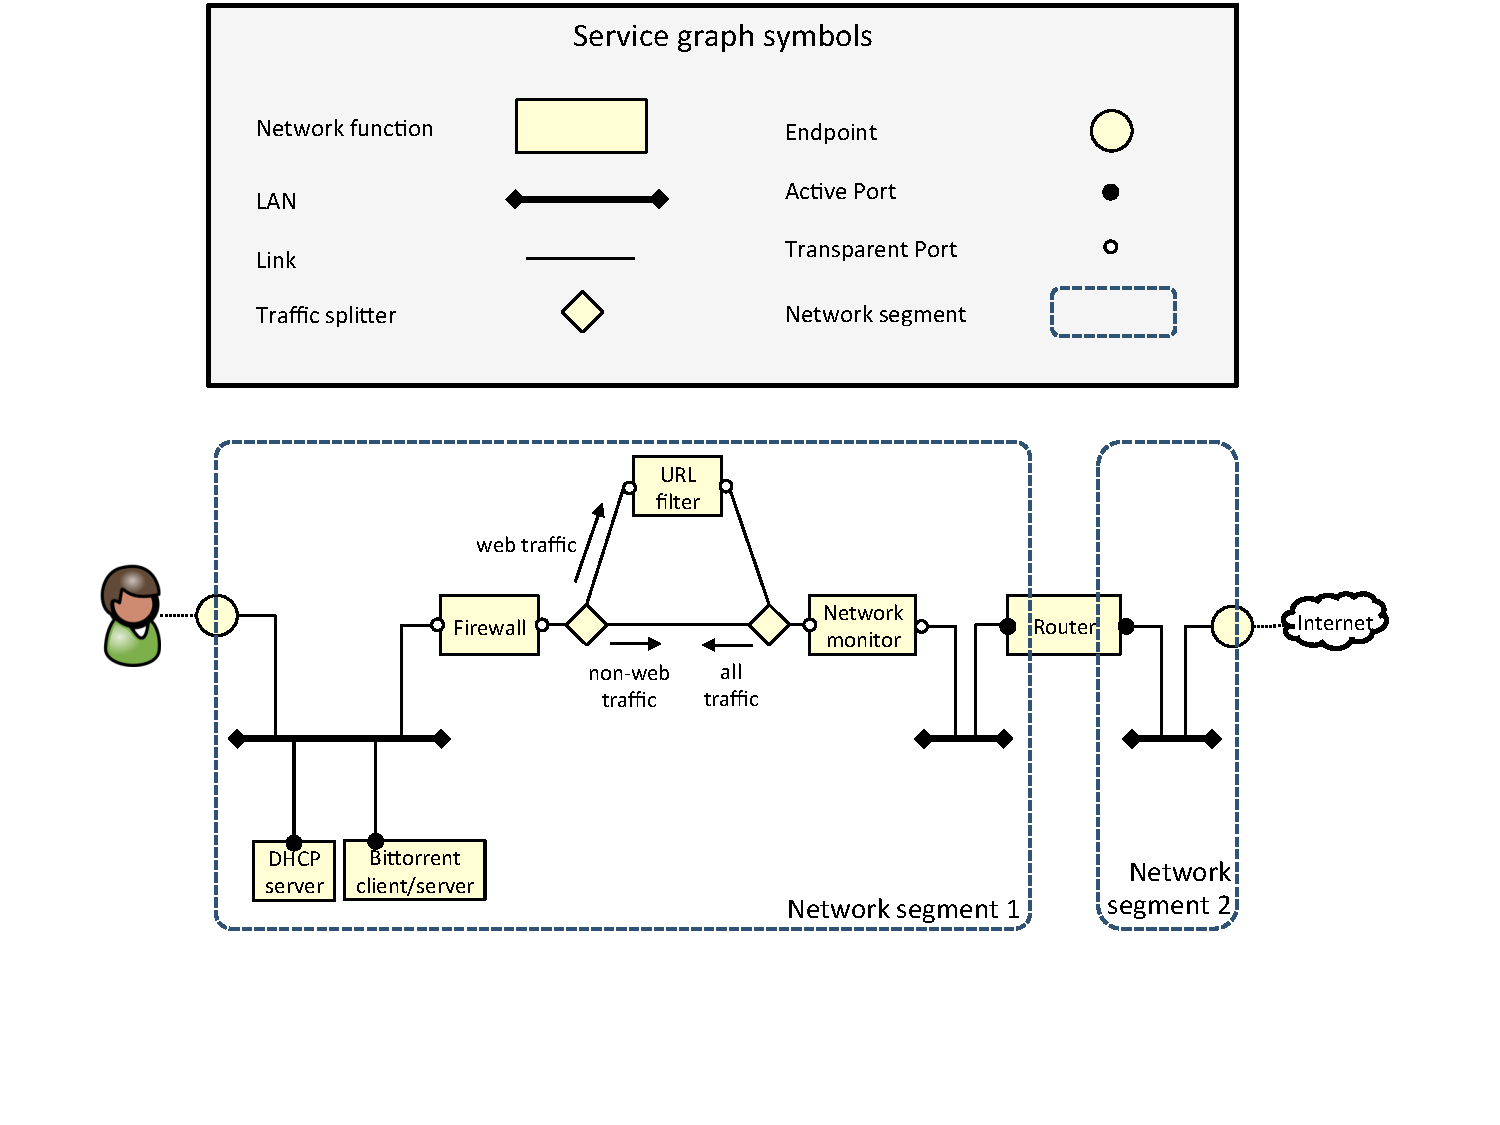
\includegraphics[clip= true, width= 0.8\columnwidth, trim= 1.5cm 3.0cm 0.6cm 0.0cm]{images/service_graph_components.pdf}
	\caption{Service graph: basic elements and example.}
	\label{fig:service_graph}
\end{figure}

From the point of view of the infrastructure, the SG consists of the set of basic elements shown in Figure~\ref{fig:service_graph}, which have been selected among the most common elements that we expect are needed to define network services.
In particular, a SG may include the following seven basic primitives:
\begin{itemize}
	\item \textbf{Network function}: it represents a functional block that may be lately translated into one (or more) VNF images. %, or to a dedicated hardware.
	%IVANO: ho rimosso il "to a dedicated hw". Perché secondo me è un dettaglio .
	%, without differentiating between transparent (e.g., network monitor) and ``active'' functions network whose network interfaces have with IP addresses, and hence that can be explicitly addressed by packets (e.g., a web server);
	Each network function is associated with a template (detailed in Section~\ref{sec:template}) describing the function itself in terms of RAM and CPU required, type of processor on which it can run (e.g., x86-64), number and types of ports, etc.
	\item \textbf{Active port}: it defines the attaching point of a network function that needs to be configured with a network-level address (e.g., IP), either dynamic or static. Packets directed to that port are forwarded by the infrastructure based on the link-layer address of the port itself (e.g., MAC address).
	\item \textbf{Transparent port}: it defines the attaching point of a network function whose associated virtual network interface card (vNIC) does not require any network-level address. If traffic has to be delivered to that port, the network infrastructure has to ``guide'' packets to it, e.g., through traffic steering elements, since the natural forwarding of the data based on link-layer addresses does not cross those ports.
	\item \textbf{Local area network (LAN)}: it represents the (logical) broadcast communication medium, i.e., the well-known primitive that allows data-link frames to be delivered to the correct recipient. The availability of this primitive facilitates the creation of complex services that include not only transparent VNFs, but also traditional host-based services that are usually designed in terms of LANs and hosts. Furthermore this provides an abstraction similar to the one available in cloud management systems, such as OpenStack, that usually offer the \textit{network} as one of the fundamental building blocks.
	\item \textbf{Point-to-point link}: it defines the logical wiring among the different components, and can be used to connect two VNFs together, 
	%implement the traffic steering between different network functions (e.g., when the output of VNF1 represents the input of VNF2), 
	to connect a port to a LAN, and more. %Links are accompanied by the proper attaching rules that define how they can be connected to the different components.
	\item \textbf{Traffic splitter/merger}: it represents a functional block that allows to split the traffic based on a given set of rules, or to merge the traffic coming from different links. For instance, it can be used to redirect only the outgoing web traffic toward an URL filter (Figure~\ref{fig:service_graph}), while the rest does not crosses that network function.
	\begin{comment}
	%IVANO: un endpoint non e' una porta fisica nel SG, così come non è un tunne gre. Poi, nel processo di lowering,  possono diventare tunnel gre o porte fisiche-
	\item \textbf{Endpoint}: it represents the external attaching point of the service graph, which can be a physical/logical port (e.g., a physical NIC, a virtual NIC or a network tunnel endpoint) or the endpoint of another service graph, if several of them have to be cascaded.
	\end{comment}
	\item \textbf{Endpoint}: it represents the external attaching point of the SG. It can be used to attach the SG to the Internet, to an end user device, but also to the endpoint of another service graph, if several of them have to be cascaded in order to create a more complex service.
	To this purpose, each endpoint is associated \textit{(i)} with an identifier, which can be used as a reference to connect two SGs together, and \textit{(ii)} with a cardinality, which indicates if the endpoint can be connected to one or many other endpoints.
\end{itemize}

In the example of SG provided in Figure~\ref{fig:service_graph}, three network functions are connected to a LAN, featuring both active (e.g., the DHCP server and the bittorrent machine, which need to be configured with IP addresses) and transparent ports (the firewall).
The outgoing traffic exiting from the firewall is received by a splitter/merge block, which redirects the web traffic to an URL filter and from here to a network monitor, while the non-web traffic travels directly from the firewall to the network monitor.
Finally, the entire traffic is sent to a router %(that originates two different network segments)
before exiting from the service graph.
It is worth noting that traffic splitter/merger modules are bidirectional and may have different behaviors in the opposite directions.
For instance, the traffic splitter/merger on the right will send \textit{all} the traffic coming from Internet to the firewall, without sending anything to the URL filter as this block needs to operate only on the outbound traffic.





As cited above, the SG also includes aspects related to the configuration of the network functions required by the service;
particularly, this information includes network aspects such as the IP addresses assigned to the active ports of the VNFs, as well as VNF-specific configurations, such as the filtering rules for a firewall.
In fact, they represent important service-layer parameters to be defined together with the service topology, %, although they are not needed to actually deploy the VNFs and virtual links in the network infrastructure.
and that can be used by the control/management plane of the network infrastructure to properly configure the service.

A SG engine may also assess formal properties on the above configuration parameters; for example, the service may  be analyzed %by some verification tools that 
to check if the IP address assigned to the VNFs active ports are coherent among each others.
To facilitate this work, the SG includes the concept of \textbf{network segment}. 
According to Figure~\ref{fig:service_graph}, each network segment is the set of LANs, links and ports that are either directly connected or that can be reached through a network function by traversing only its transparent ports. 
Hence, it corresponds to an extension of the broadcast domain, as in our case data-link frames can traverse also network functions (through their transparent ports), and it can be used to check that all the addresses (assigned to the active ports) of the same network segment belong to the same IP subnetwork.
As shown in the picture, a network segment can be extended outside of the SG; for instance, if no L3 device there exists between an end user terminal and the graph endpoint, the network segment also includes the user device.





As a final remark, the configuration parameters for the network functions, as well as the possibility of assessing formal properties on them, are out of the scope of this paper and will be investigated in our future work.
\begin{comment}


\section{Service graph}
%\chapter{Service graph}
\label{chap: Service graph}
\label{sec:service_graph}

In our topology of service we defined a model used to represent an high level of service that the user asks to the network, this is called Service graph. It consists of the set of basic elements shown in Figure \ref{fig:service_graph_components}. 
\begin{figure}[h]
	\centering
	% left bottom right top
	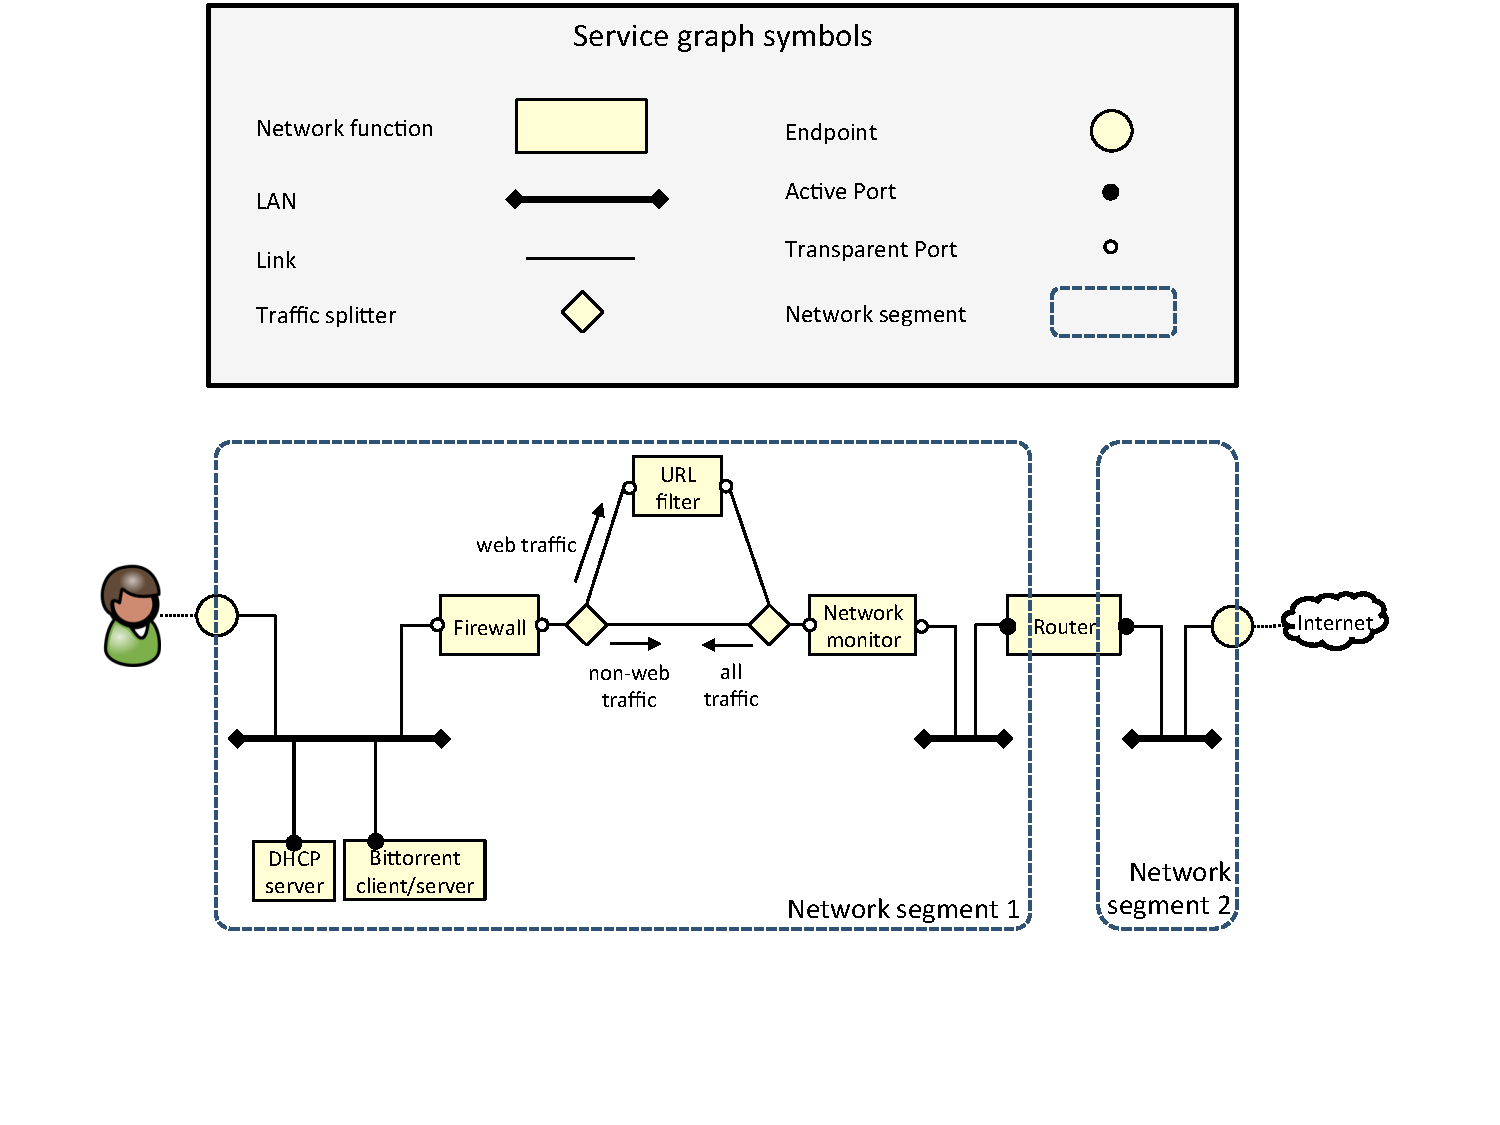
\includegraphics[clip= true, width= \columnwidth]{images/service_graph_components.pdf}
	\caption{SG - Service graph components}
	\label{fig:service_graph_components}
\end{figure}
These primitives have been selected among the most common elements that we expect are needed by the users to create their own network service.
In particular, a SG may include the following seven basic primitives:
\begin{itemize}
	
	\item \textbf{Network functions}: it represents a functional block that may be lately translated into one (or more) VNF images. It can arbitrarily create/delete packets, change the packet content (e.g., protocol headers/data), and determine the output port where to send it. The internal behavior of this functional block is not known by the other entities and it is arbitrarily determined by the service (e.g., network function) itself.
	
	\item \textbf{Active port}: it defines the attaching point of a network function that needs to be configured with a network-level address (e.g., IP), either dynamic or static. Packets
	directed to that port are forwarded by the infrastructure based on the link-layer address of the port itself (e.g., MAC address).
	
	\item \textbf{Transparent port}: it defines the attaching point of a network function whose associated virtual network interface card (vNIC) does not require any network-level address. If traffic has to be delivered to that port, the network infrastructure has to “guide” packets to it, e.g., through traffic steering elements, as the natural flow of data, which is based on link-layer addresses, does not cross those ports.
	
	\item \textbf{Local area network (LAN)}: it represents the (logical) broadcast communication medium, i.e., the well-known primitive that allows data-link frames to be delivered to the correct recipient. The availability of this primitive facilitates the creation of complex services, as network-savvy people still tend to think about networks and hosts.
	
	\item \textbf{Point-to-point link}: it defines the logical wiring among the different components. It can be used to implement the traffic steering between different network functions (e.g., when the output of VNF1 represents the input of VNF2), to connect an active port to a LAN, and more. Links are accompanied by the proper attaching rules that define how they can be connected to the different components.
	
	\item \textbf{Traffic splitter/merger}: it represents a functional block that allows to split the traffic based on a given set of rules, or to merge the traffic coming from different links. For instance, it can be used to redirect only the outgoing web traffic toward an URL filter (Figure 2), while the rest does not crosses that network function.
	
	\item \textbf{Endpoint}: it represents the external attaching point of the SG. It can be used to attach the SG to the Internet, to the user device, but also to the endpoint of another service graph, if several of them have to be cascaded.
	
\end{itemize}

Moreover, the SG can also include network-layer information such as IP address. In fact, although IP addresses are not needed at all when we need to deploy VNFs and virtual links in the network infrastructure, they may represent an important service-layer parameter for users, who may need to define them together with the service topology.
In the example of SG provided in Figure 2, three network functions are connected to a LAN, featuring both active (e.g., the DHCP server and the bittorrent machine, which need to be configured with IP addresses) and transparent ports (the firewall). The outgoing traffic exiting from the firewall is received by a splitter/merge blocks, which redirects the web traffic to an URL filter and from here to a network monitor, while the non-web traffic travels directly from the firewall to the network monitor. Finally, the entire traffic is sent to a router (that originates two different network segments) before exiting from the service graph.
It is worth noting that traffic splitter/merger modules are bidirectional and may have different behaviors in the opposite
directions. For instance, the traffic splitter/merger on the right will send all the traffic coming from Internet to the firewall, without sending anything to the URL filter as this block needs to operate only on the outbound traffic.
The required service, before being actually instantiated on the network, may need to be analyzed by some verification tools, which check if the SG satisfies some properties. To facilitate the work of these tools, we defined the network segment element, which is shown in Figure 2. As evident from the picture, each network segment is the set of LANs, links and ports that are either directly connected or that can be reached through a network function by traversing only its transparent ports. Hence, it corresponds to an extension of the broadcast domain, as in our case data-link frames can traverse also network functions (through their transparent ports), and it can be used to check that all the addresses (assigned to the active ports) of the same network segment belong to the same IP subnetwork. It is worth noting that the network segment may also include the user terminal, if no L3 device there exists between the terminal itself and the graph endpoint, as shown in the left of the picture.
As a final remark, in order to facilitate the service creation, we expect that the user is provided with a graphical interface that makes available the above elements (except the network segments, generated by the system), and that is integrated with an AppStore-like marketplace that enables uses to select a precise function among the many available.
\end{comment}

\subsection{Cascading service graphs}
\label{sec:ep_cascade}

As introduced above, the SG endpoints are associated with multiple parameters that are used to connect SGs together (cascading graphs). 
Particularly, the name is the foundation of the SG attaching rules, indeed  %as only the endpoints with the same identifier (shown with the same color in Figure ) can be attached together.
the logic that connects the endpoints is demanded to service layer but is done on the basis of their names.

The cardinality specifies if that endpoint can be used to connect the graph with one or many other graphs, i.e., to implement a one-to-one or a one-to-many connection. Finally, the optional ingress matching rule indicates which traffic is allowed to enter into the graph through that particular endpoint, e.g., only the packets with a specific source MAC address.

The cardinality specifies if that endpoint is used to connect the graph with one or many other graphs, i.e., to implement a one-to-one or a one-to-many connection. Finally, the optional ingress matching rule indicates which traffic is allowed to enter into the graph through that particular endpoint, e.g., only the packets with a specific source MAC address.

The rules that define how to connect several graphs together change according to both the cardinality of the endpoints involved and to the presence of an ingress matching rule on such endpoints. While the case in which only two endpoints have to be connected (i.e., direct connection) does not present significant issues, Figure~\ref{fig:endpoints} presents two examples in which an one-to-one endpoint (in the SG on the left) must be connected to a common graph through its one-to-many endpoint. In this example we consider a first packet flowing from the left to the right, while the return packet follows the opposite path.

\begin{figure} %[h]
	\centering
	% left bottom right top
	\includegraphics[clip= true, width= 0.9\columnwidth, trim= 0.1cm 1.2cm 0cm 0.0cm, page= 19]{images/Pictures_definitivo.pdf}
	\caption{Connection of many user SGs to a single ISP SG.}
	\label{fig:endpoints}
\end{figure}

Example 1 in Figure~\ref{fig:endpoints} presents two egress endpoints that are associated with a ingress matching rule specifying which traffic must enter into the graph through that endpoint. This ingress matching rule must be used, in case of return traffic, to deliver the desired packets to the correct graph, notably HTTP traffic to the “HTTP-SG” and FTP traffic to the “FTP-SG”. This is achieved by transforming the ingress endpoint of the “TCP-SG” into the set of components enclosed in the green shape of Example 1(b), notably a traffic splitter/merger module attached with many new endpoints, each one connected to a different graph. This way, the common “TCP-SG” will be able to dispatch the packet answers to the proper graph.
Example 2 in Figure 4 shows instead the case in which the egress endpoints are not associated with any ingress matching rule, which makes impossible to determine the right destination for the packets on the return path as a traffic splitter/merger module cannot be used in the “ISP-SG” to properly dispatch the traffic among them. In this case, the ingress endpoint of the common “ISP- SG” is transformed into a LAN connected to several new endpoints, each one with one-to-one cardinality and dedicated to the connection with a single other graph. This way, thanks to the MAC-based forwarding guaranteed by the LAN, the “ISP-SG” can dispatch the return packets to the proper graph, based on the MAC destination address of the packet itself.
%
%
%
%
\begin{comment}
The SG and FG models proposed in this thesis allow the concatenation of many service graphs through the graph endpoints.
To this purpose, each endpoint is associated with an unique identifier and a cardinality, indicating if that endpoint can be used to connect the graph with one or many other graphs, i.e., to implement a \texttt{one-to-one} or a \texttt{one-to-many} interconnection.
Then, before the FG is given to Infrastructure layer, the endpoints are manipulated as follows.
If the connection is between endpoint never connected until now (\texttt{one-to-one} connection) endpoints are let unmodified, while if at least one of endpoints evolved  in the connection are already connected with an other graph (\texttt{one-to-many} connection),  endpoint is connected with a LAN connected with several new endpoints, each one marked as \texttt{one-to-one}, and that will be dedicated to the connection to a single other graph.

To better understand, consider the use case under analysis, which requires that each end user SG is cascaded with a common graph defined by the ISP, so that: \textit{(i)} the packets generated by the end users are processed in the ISP graph before going towards the Internet; \textit{(ii)} the packets coming from the Internet are first handled by the ISP graph, which is then able to provide them to the proper user SG.
%Hence, the following of this section details how these inter-SG connections are implemented in our service layer, by using as an example our use case.

Particularly, referring to Figure~\ref{fig:endpoints}(a), the \textit{egress} endpoint of each user SG must be connected to the \textit{ingress} endpoint of the ISP SG.
As a consequence, the \textit{egress} endpoint of the user graph is marked as \texttt{one-to-one}, while the \textit{ingress} endpoint of the ISP graph is marked as \texttt{one-to-many}. %, since it must be connected to several end user graphs\footnote{Remember, in fact, that the ISP graph is shared among all the end users.}.
Hence, the service layer replaces this last endpoint with several new endpoints connected to a LAN, as depicted in Figure~\ref{fig:endpoints}(b).

\begin{figure} %[h]
	\centering
	% left bottom right top
	\includegraphics[clip= true, width= 0.9\columnwidth, trim= 0.1cm 1.2cm 0cm 0.0cm, page= 19]{images/Pictures_definitivo.pdf}
	\caption{Connection of many user SGs to a single ISP SG.}
	\label{fig:endpoints}
\end{figure}


According to Figure~\ref{fig:endpoints}(c), when a user SG is going to be deployed, its endpoint are not expanded, since they are marked as \texttt{one-to-one}.
However, the SLApp creates a logical connection between the \textit{egress} endpoint of the graph itself and one of the new endpoints of the ISP SG.
This way, the orchestration layer (which has no information on the use case implemented by the service layer) knows that the traffic going towards/coming from the Internet must be processed by the ISP SG after/before going towards its final destination, %and that traffic coming from the Internet must enter in the ISP SG before being handled by the service defined by a specific user, 
and hence can instruct the infrastructure layer to create the proper links.


\end{comment}


\section{Forwarding graph}
\label{sec:forwarding_graph}

The SG provides an high level formalism to define network services, but it is not adequate to be deployed on the physical infrastructure of the network, since it does not include all the details that are needed by the service to operate.
Hence, it must be translated into a more resource oriented representation, namely the \textbf{forwarding graph (FG)} (Chapter~\ref{chap:the_state_of_the_art}), through the so called \textbf{lowering process}.

The differences between the SG and the FG, together with the steps needed to transform a the first representation into the second one (i.e., the lowering process), are shown in Figure~\ref{fig:graphs} and discussed in the following:


\begin{figure}[h]
	\centering
	% left bottom right top
	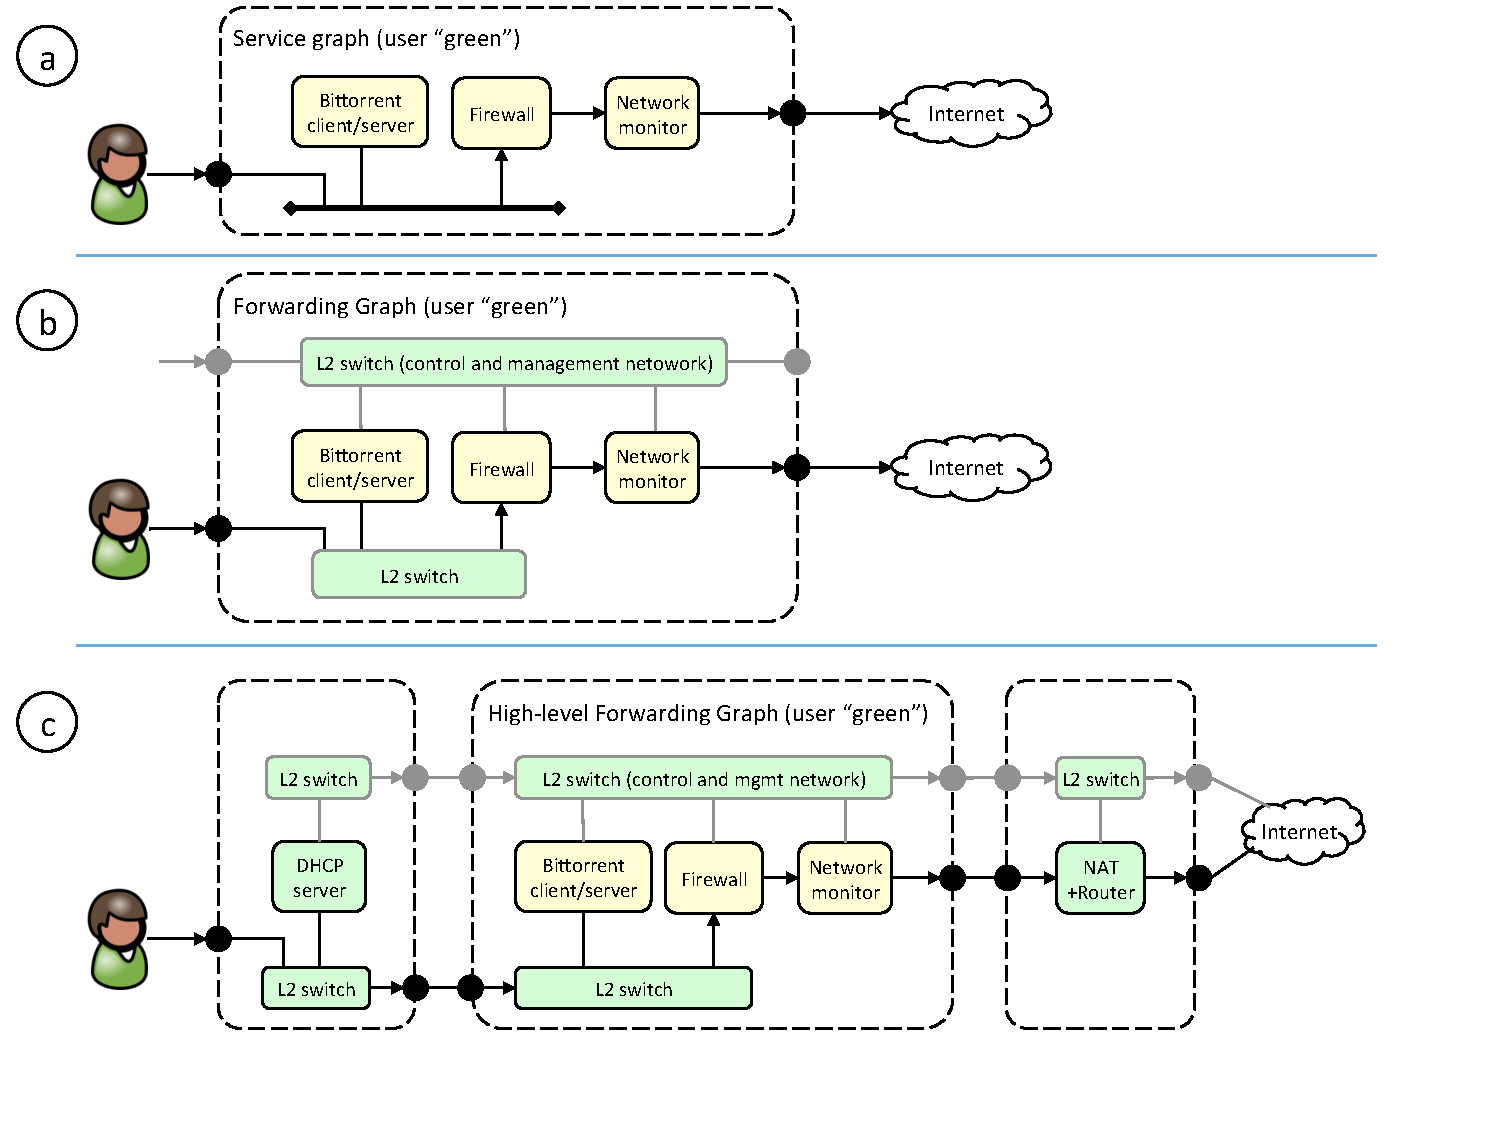
\includegraphics[clip= true, width= 0.8\columnwidth, trim= 0.0cm 1.4cm 1.2cm 0.0cm]{images/NF-FG.pdf}
	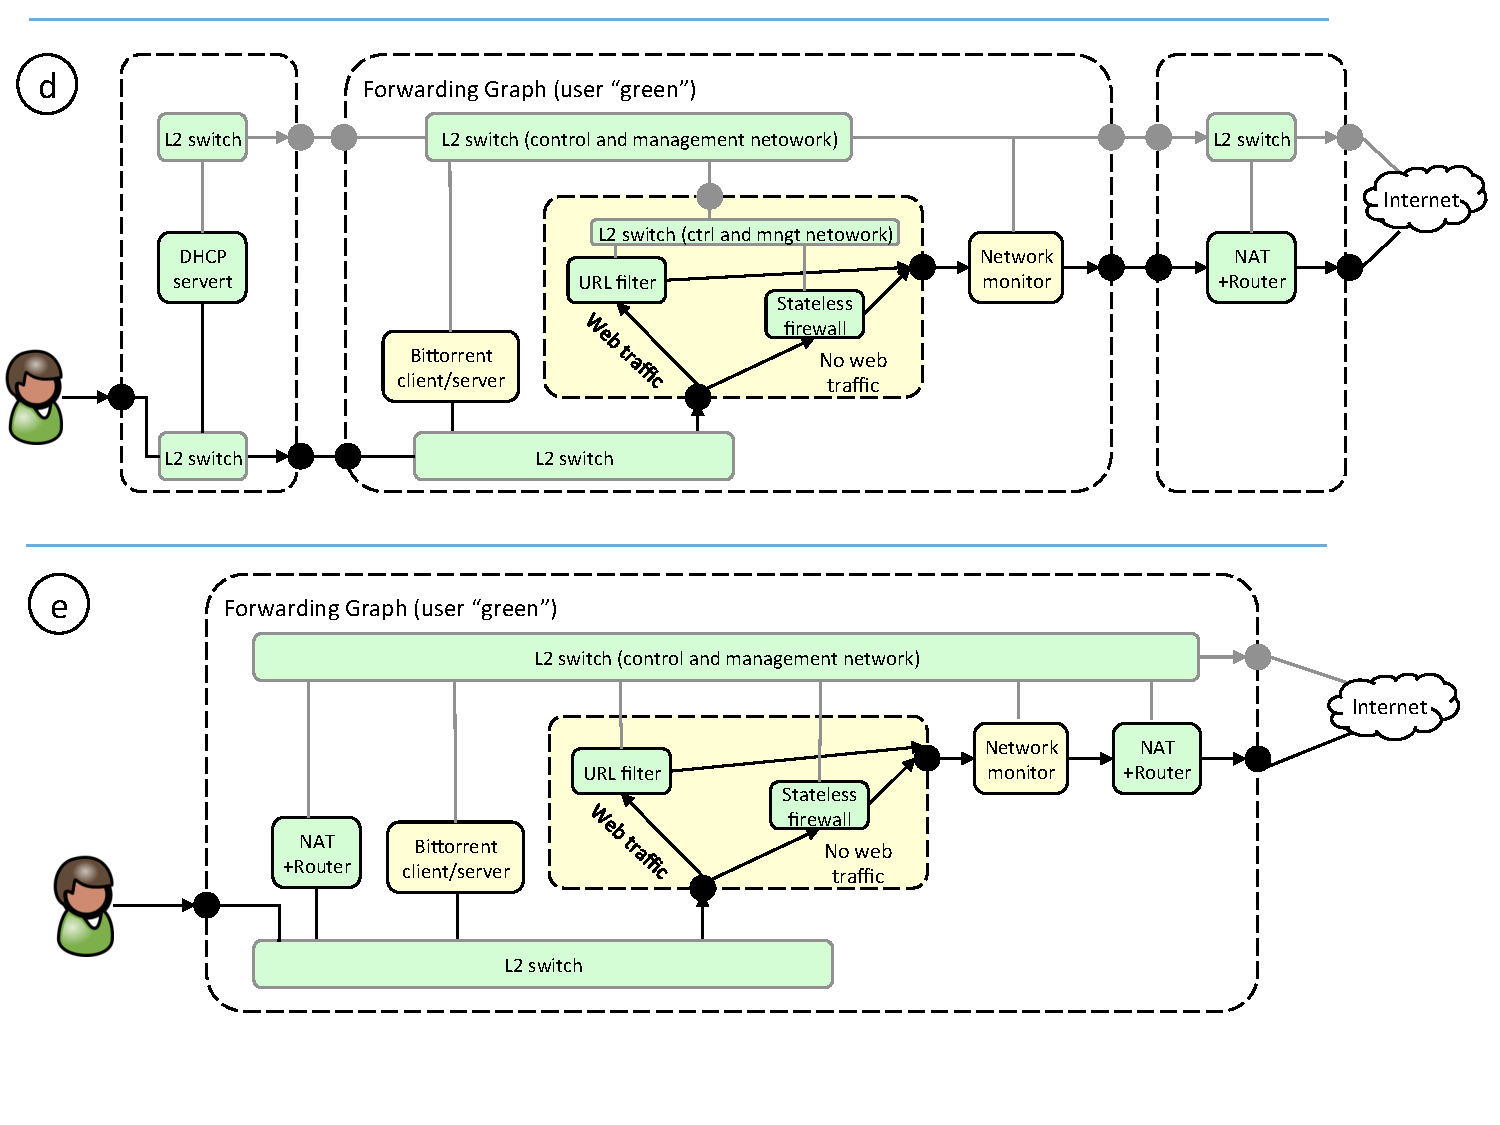
\includegraphics[clip= true, width= 0.8\columnwidth, trim= 0cm 1.8cm 0.2cm 0.0cm]{images/NF-FG2.pdf}
	\caption{From the service graph to the forwarding graph: the lowering process.}
	\label{fig:network_function_forwarding_graph}
	\label{fig:graphs}
\end{figure}

%
\begin{itemize}
	\item  \textbf{Control and management network expansion}: the service is enriched with the ``control and management network'', which may be used %only be accessible by some actors (e.g., the network provider) in order 
	to  properly configure  the VNFs of the graph.
	In fact, most network functions require a specific vNIC dedicated to the control/management operations; although this may be an unnecessary detail for the user requiring the service, those network connections have to be present in order to allow the service to operate properly. 
	An example of this step is evident by a comparison between Figure~\ref{fig:graphs}(a) and  Figure~\ref{fig:graphs}(b), in which a control/management network consisting of a L2 switch VNF has been added to the graph\footnote{It is worth pointing out that, although the control and management network in Figure~\ref{fig:graphs}(b) only includes a L2 switch, this network could also include other VNFs, such as a firewall.}.
	\item \textbf{LAN expansion}: all the LANs expressed in the SG are replaced with VNFs implementing the MAC learning switch.
	This step is again shown in Figure~\ref{fig:graphs}(b), and it is needed in order to translate the abstract LAN element available in the SG into a VNF actually realizing the broadcast communication medium.
	\item \textbf{Service enrichment}: the graph is analyzed and enriched with those functions that have not been inserted in the SG, but that are required for the correct implementation and delivery of the service.
	As shown in the example provided in Figure~\ref{fig:graphs}(c), if the graph analysis determines, for instance, that the graph does not include a DHCP server and does not terminate with a VNF acting as a router and as a NAT,  these functions are automatically added at this step of the lowering process.
	\item \textbf{VNFs expansion}: according to its template described in Section~\ref{sec:template}, a VNF may be expanded in a number of VNFs, properly connected in a way to implement the required service.
	As an example, the firewall in Figure~\ref{fig:graphs}(c) is replaced, in Figure~\ref{fig:graphs}(d), with a subgraph composed of an URL filter only operating on the web traffic, while the non-web traffic is delivered to a stateless firewall.
	As evident, the ports of the ``original'' VNF are now the endpoints of the new subgraph, which also have a control network dedicated to the new VNFs.
	Moreover, these new VNFs are in turn associated with a template, and can be recursively expanded in further subgraphs; this is an implementation of the ``\textit{recursive functional blocks}'' concept provided by NFV definition in ETSI standard (Chapter~\ref{chap:the_state_of_the_art}).
	\item \textbf{Consolidation}: it consists in the replacement, with a single VNF, of those VNFs implementing the L2 forwarding that are connected together, in order to limit the resources required to implement the LANs on the physical infrastructure.
	An example of this step is provided in Figure~\ref{fig:graphs}(e).
	\item \textbf{Endpoint translation}: it is the last step of the lowering process, in which the graph endpoints can be converted in: physical ports of the node on which the graph will be deployed; tunnel endpoints (e.g., GRE) used to connect two pieces of the same service but on different physical servers; endpoints of another FG, if many graphs must be connected together in order to create a more complex service.
	\item Finally, the \textbf{flowrules definition} concludes the lowering process. In particular the connections among the VNFs, as well as the traffic steering rules (expressed through the traffic splitter/merger components in the SG) can be represented with a sequence of ``flowrules'' (Listing~\ref{lst:NF-FG_flowrule}), each one indicating which traffic has to be delivered to a specific VNF (on a given port of that VNF), or the physical port/endpoint through which the traffic has to leave the graph. 
	
	\lstinputlisting[label=lst:NF-FG_flowrule, language=python, caption={Example of flourule associated to specific VNF port.}]{code/NF-FG_example_vnf_flowrules.txt}
	
	
	The flowspec supports all the fields defined by Openflow 1.0~\cite{of10} (although new fields can be defined), while the action can refer to a forwarding of packets either through a physical port, through a logical endpoint, or through a port of a VNF. 
	Hence, the FG is actually a generalization of the Openflow data model that specifies also the functions that have to process the traffic into the node, in addition to define the (virtual) ports the traffic has to be sent to.
	
	
	
\end{itemize}










\begin{comment}


\section{Forwarding graph}
\label{sec:forwarding_graph}

\begin{figure}[h]
	\centering
	% left bottom right top
	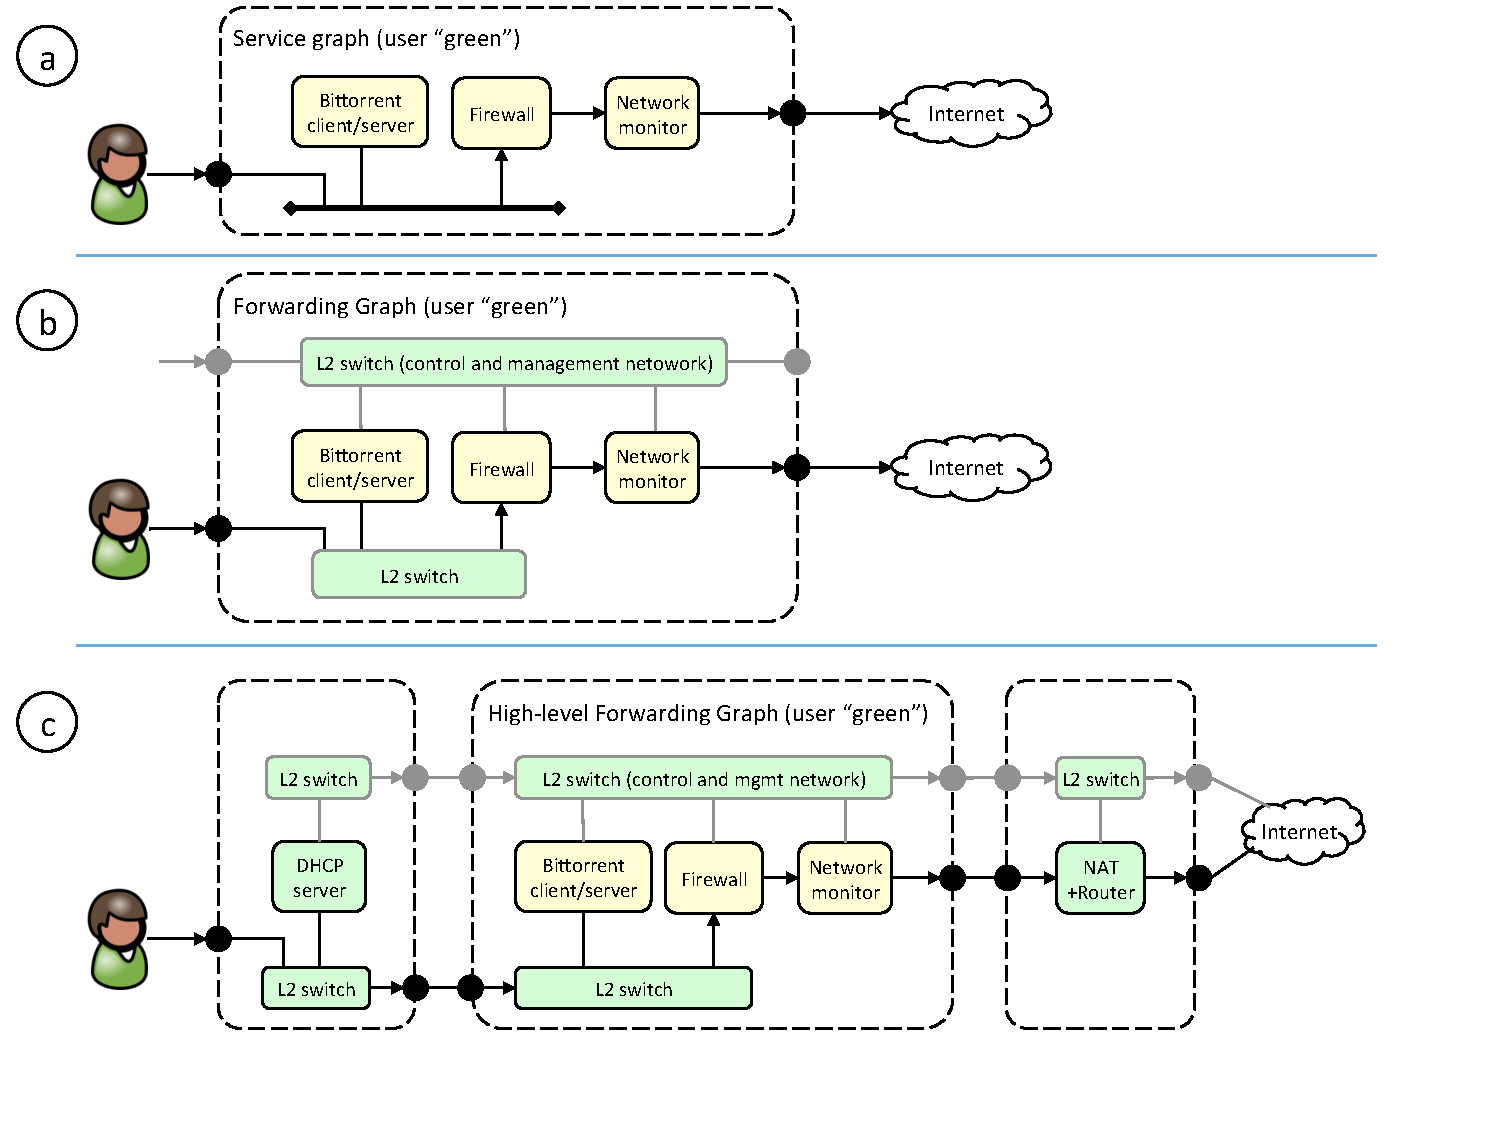
\includegraphics[clip= true, width= 0.8\columnwidth, trim= 0.0cm 1.4cm 1.2cm 0.0cm]{images/NF-FG.pdf}
	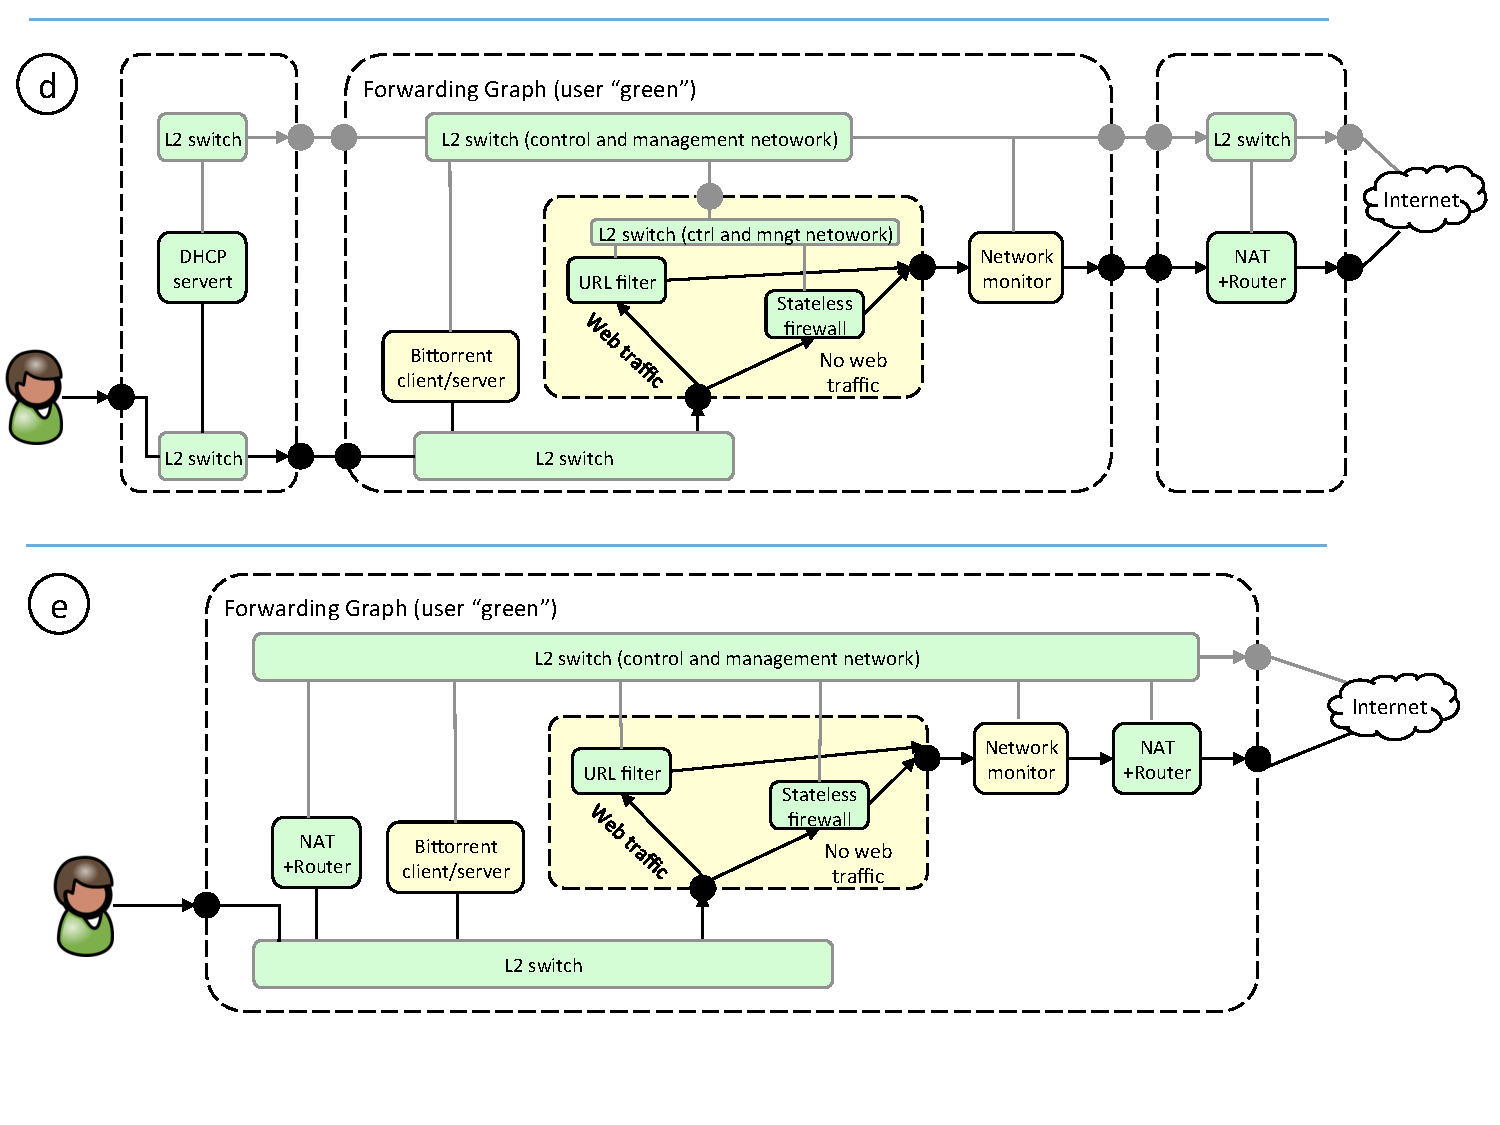
\includegraphics[clip= true, width= 0.8\columnwidth, trim= 0cm 1.8cm 0.2cm 0.0cm]{images/NF-FG2.pdf}
	\caption{From the service graph to the forwarding graph: the lowering process.}
	\label{fig:network_function_forwarding_graph}
	\label{fig:graphs}
\end{figure}

The SG just introduced provides to the users an high level formalism to define their services, but it is not adequate to be deployed on the physical infrastructure of the network. Hence, it must be lowered into a more resource oriented representation, namely the \textbf{forwarding graph (FG)}. Although, similar to the SG, this formalism provides an end-to-end description of the VNFs involved in the service itself and their logical connections, the SG does not include all the details that are needed by the service to operate, and hence several differences there exist between the two representations. These differences, together with the steps needed to transform a SG into a FG (i.e., to implement the \textbf{lowering process}) are shown in Figure \ref{fig:network_function_forwarding_graph} and discussed in the following of this section.
First of all, most network functions require a specific vNIC dedicated to the control/management operations, which may be accessible only by the network provider. Although this is an unnecessary detail for the user, those network connections have to be present in order to allow the service to operate properly. Hence, the first step of the logic that translates the SG into the actual building blocks has to complete the FG with the control and management network, as evident by a comparison between Figure \ref{fig:network_function_forwarding_graph}(a) and Figure \ref{fig:network_function_forwarding_graph}(b).The latter picture also shows the second step of the lowering process, which consists in the replacement of the LANs expressed in the SG with VNFs implementing the MAC learning switch, called “L2 switch” in the figure.
Figure \ref{fig:network_function_forwarding_graph}(c) shows instead the third step of the process to translate the SG into a FG, which consists in the enrichment of the service expressed by the user with a number of VNFs needed for the correct implementation of the service itself. For example, the picture shows that the user graph is connected to the left with a first graph containing a DHCP server attached to a switch, while to the right it is connected with a second graph that consists of a VNF implementing a router and a NAT. The SG considers a network function like a generic functional block, hence missing low-level details such as the number (and types) of software images that need to be instantiated. For instance, a VNF expressed in the SG may be expanded in a number of VNFs in the FG, properly connected in a way to implement the required service: this is the fourth step of the lowering process. As an example, the firewall in the Figure \ref{fig:network_function_forwarding_graph}(c) is replaced, in Figure \ref{fig:network_function_forwarding_graph}(d), with a subgraph composed of an URL filter only operating on the web traffic, while the non-web traffic is provided to a stateless firewall. It is worth noting that the ports of the “original” VNF are now the endpoints of the new subgraph, which also have a control network dedicated to the new VNFs.
Finally, the last step of the lowering process consists in the consolidation of the three pieces of graph into a single one, as shown in Figure \ref{fig:network_function_forwarding_graph}(e). In this step, the VNFs implementing the L2 forwarding and that are connected together are replaced with a single VNF, in order to limit the resources required to implement the LANs on the physical infrastructure.


\lstinputlisting[label=lst:NF-FG_flowrule, language=python, caption={Example of flourule associated to specific VNF's port}]{code/NF-FG_example_vnf_flowrules.txt}


In addition, all the connections among the VNFs and the traffic steering rules (expressed through the traffic splitter/merger components in the SG) originate a sequence of “flowrules” associated to each VNFs port (Listing \ref{lst:NF-FG_flowrule}), each one indicating which traffic has to be delivered to a specific VNF (on a given port of that VNF), or the endpoint through which the traffic has to leave the graph. The action can refer either to an endpoint or to a port of a VNF, while the matches in flow spec supports all the fields defined by Openflow 1.0 (although new fields can be defined). In this respect, we can consider the FG as a generalization of the Openflow data model that specifies also the functions that have to process the traffic into the node, in addition to defining the (virtual) ports the traffic has to be sent to.
Furthermore in the current implementation of FG the labels associated in the SG to endpoints shown in Figure~\ref{fig:endpoints} become ingoing rules for the VNFs ports linked to the endpoints.

As a final remark, the FG does not specify yet low level details such as the physical node on which the service will be deployed, as well as the reference to the precise physical/virtual interfaces needed by the VNF to operate, replaced by generic entry/exit points for the graph.
\end{comment}

\subsection{Structure of the FG}
This section contains a detailed analysis of the forwarding graph description.

The notation used to describe the forwarding graph is JSON (JavaScript Object Notation). A first level description of FG is given by Listing \ref{lst:NF-FG_example}.

\lstinputlisting[label=lst:NF-FG_example, language=python, caption={High-level view of FG.}]{code/NF-FG_example.txt}

The information contained in FG is: \textit{(i)} a list of virtual network functions, \textit{(ii)} a list of endpoints, \textit{(iii)} a unique identifier of the FG.
With regards to VNFs as shown in Listing \ref{lst:NF-FG_example_vnf}, they are characterized by a \texttt{vnf\_descriptor}, a list of \texttt{ports}, a \texttt{name} and an \texttt{id}.
\lstinputlisting[label=lst:NF-FG_example_vnf, language=python, caption={High-level view of VNFs.}]{code/NF-FG_example_vnf.txt}

% Ports

The ports described in VNFs JSON object are the ports actually used by a VNF, while a complete list of ports available for a VNF is contained in the VNF template (Section \ref{chap:VNFdescriptor}). Now we are going to analyze each field of the \texttt{VNFs} element in detail.

The \texttt{id} is an unique identifier of the VNF in the FG, while the \texttt{name} identify the type of VNF.
The \texttt{vnf\_descriptor} is an URL containings a manifest of the virtual network function that are (described in section \ref{chap:VNFdescriptor}).
The \texttt{port} list that are shown in the Listing \ref{lst:NF-FG_example_vnf_ports} contains an \texttt{id}, an \texttt{ingoing\_label}, and an \texttt{outgoing\_label}.
The port \texttt{id} is composed of two different parts, the part before the column identify the label (this one will be explained in section \ref{chap:VNFdescriptor}) of the port, the second part is an id for all ports with same label.  The \texttt{outgoing\_label} contains flow rules that only identify outgoing traffic from the port, while \texttt{ingoing\_label} contains flow rules only for ingoing traffic to that port.
While the outgoing labels are mandatory, the ingoing labels is needed only when a port is connected to an endpoint, since the endpoint does not have any flowrule associated.
In addiction, flow rules contained in an ingoing label have an addictional field to identify the endpoint from which the traffic comes. This field is called \texttt{ingress\_endpoint} and it is a leaf of flowspec object (line 10 of Listing~\ref{lst:NF-FG_flowrule}). Finally the flowrule object, as discussed before (Listing~\ref{lst:NF-FG_flowrule}) contains a list of matches on packets and the relative action. 


\lstinputlisting[label=lst:NF-FG_example_vnf_ports, language=python, caption={High-level view of ports}]{code/NF-FG_example_vnf_ports.txt}

It is worth noting that all the flow rules of a single port must forward the totality of traffic, hence, a rules of specific port cannot purge the traffic, and if we want to drop some kind of traffic we must do that in a VNF. Therefore it is clear that, the only type of actions can be ``output''.

% Endpoint

The \texttt{endpoints} (Listing~\ref{lst:NF-FG_example}) are the termination of graph. In the FG instead of SG, the endpoints can assume various characterizations like for example: \textit{(i)} tunnel termination, \textit{(ii)} physical port or \textit{(iii)} virtual port. For instance, the example in Listing \ref{lst:endpoint} shows an endpoint that is actually a physical port called "ge0". This characterization is needed to effectively connect graphs among each other and map the endpoint concept on physical resources.
\lstinputlisting[label=lst:endpoint, language=python, caption={NF-FG - Example of endpoint definition.}]{code/endpoint.txt}

With regard to name, it provides a tool to implement the logic of connection between graphs, together with a further field called \texttt{connection\_cardinality}, which specify the type of connection. It can assume two different values: \texttt{(i)} \texttt{one-to-many} or \texttt{(ii)} \texttt{many-to-many} as specified in Section~\ref{sec:ep_cascade}.
%that is present only when we should connect more than one endpoint to this endpoint. It consist of an id of a layer 2 switch VNF that are connected to this endpoint, the switch is used to route the packet in the right way. Therefore in this case the really endpoints (where the other graphs are really connected) are attached to other ports of the layer 2 switch link in figure \ref{}. This when necessary, is added by the service layer \ref{}.













\subsection{Operations}
As stated above, several actions can be executed on a FG. Particularly, these actions are: \textit{(i)} endpoint connection like in the passage between Figure \ref{fig:network_function_forwarding_graph}(d) and Figure \ref{fig:network_function_forwarding_graph}(e)  and \textit{(ii)} the node expansion like in the passage between Figure \ref{fig:network_function_forwarding_graph}(c) and Figure \ref{fig:network_function_forwarding_graph}(d).

\subsubsection{Connection}
The connection between different graphs is made through the endpoints, which represent the ingress/exit point from the graph. The connection depends on the service layer application implementation, indeed there are two possible types of connections: \textit{(i)} the graphs are logically connected, so the output of this operation is a new graph that doesn't have anymore the endpoints used for the connection, or \textit{(ii)} the connection operation preserve the endpoints used for the connection, so they can be used again for an other connection. The former case is evident by comparing  Figure~\ref{fig:network_function_forwarding_graph}(d) and Figure~\ref{fig:network_function_forwarding_graph}(e), while the latter case represents the situation in which the results of the operation are in turn two different graphs 
that communicate with each other through the endpoint (e.g. user graph connected to an ISP graph).
\begin{comment} 
\fabio{This connection is different depending on two possible situation: (i) the graphs should be logically connected (the union of these graphs represents only one graph belonging to single owner), (ii) the graphs should be connected and instantiated on the same host  or on different hosts (the union of these graph represent however two graphs belonging to two different owner). In the first case the connection is only logically and visible only at orchestration level and at the end of this operation the endpoint disappear, instead in the second case the connection is performed between graphs of two different users, this time it is a real connection and the endpoint must be characterized. }
\end{comment}
%
%
The connection process requires Cartesian product of the ingoing labels of ports directly connected to the endpoints involved in the operation of one graph and the outgoing label of specular ports on the other graph. In this way problem can arise in the resulting flows (especially with regard to the priorities, seen that we use Openflow in our implementation).

\paragraph{The flow rule merging problem}
\label{chap:the_merging_problem}

Endpoints connection has a problem merging the flowrules. Analyzing the problem, only the intersection between flow rules should remain after the connection of two endpoints, so when we try to connect two ports that were connected to two endpoints, if the intersection of the outgoing rules towards the endpoint of one and the ingoing rules from the endpoint of the other is null, then this two ports shouldn't be connected. To better explain this problem, consider the example shown in Figure \ref{fig:NF-FG_the_merging_problem}.
\begin{figure}[h]
	\centering
	% left bottom right top
	\includegraphics[clip= true, width= \columnwidth, trim= 0cm 2cm 0cm 0cm, page= 37]{images/Pictures_definitivo.pdf}
	\caption{The merging problem.}
	\label{fig:NF-FG_the_merging_problem}
\end{figure}
As evident the connection between VNF3 and VNF1 should disappear since there are not traffic matches in common. Furthermore, the traffic from VNF4 to VNF2 becomes the intersection between the totality of traffic (*) (prensent on the rule that bring the traffic from VNF4 to endpoint)  and the totality of traffic less tcp traffic on port 80 (*-TCP80) (prensent on the rule that bring the traffic from endpoint to VNF2), that is *-TCP80. 


\begin{figure}[h]
	\centering
	% left bottom right top
	\includegraphics[clip= true, width= \columnwidth, trim= 0cm 0.2cm 0cm 0cm, page= 38]{images/Pictures_definitivo.pdf}
	\includegraphics[clip= true, width= \columnwidth, trim= 0cm 10cm 0cm 0.2cm, page= 39]{images/Pictures_definitivo.pdf}
	\caption{NF-FG - The merging problem.}
	\label{fig:NF-FG_the_merging_problem_2}
\end{figure}


The biggest problem related to the fusion of rules is to assign the right priority to the traffic. In our formalism is not possible to express the rule \textit{all traffic \textbf{except} tcp traffic on port 80}. To better understand consider the high part of Figure~\ref{fig:NF-FG_the_merging_problem_2} where the following rules are expressed on a port of VNF3: one that brings traffic to VNF5 that has matches all TCP traffic on port 80, and having a certain priority, and the other rule for traffic to the endpoint  which matches all the traffic having a lower priority than the other. Hence, the priorities of the rules play a fundamental role in the actual construction of the network topology, and allow to realize the rule ``all traffic less''.
In the example shown in Figure~\ref{fig:NF-FG_the_merging_problem_2}, are included the  priority. As we can see from the ``FG final 1'' of Figure~\ref{fig:NF-FG_the_merging_problem_2}, assigning to flow rules on the port of VNF1 the priority of the flow rules of ``FG one'' the flow towards VNF5 is never used because it more specific than the other and have the lowest priority. Furthermore using, for all pair of flows generated from the connection, the priority of starting FG we will have the same priority to multiple rules. In this case, is not guaranteed the direction of flow (``FG final 2'' in the bottom right of Figure~\ref{fig:NF-FG_the_merging_problem_2}). Hence the right choice is more complicated of the simple copy of priority and in certain cases we should change accordingly a lot of rules (``FG final 3'' in the bottom of Figure~\ref{fig:NF-FG_the_merging_problem_2}). For these reasons and because this is not the core of the thesis the code implemented has the limitation of handle
only \textit{1 to 1} or \textit{1 to n} rules fusion, so the case \textit{n to n} like for VNF3 in Figure~\ref{fig:NF-FG_the_merging_problem_2} is not taken into account.

\subsubsection{Expansion of a VNF}
The terms VNF expansion means to replace a VNF with a new graph, in which the endpoints of the graph  correspond to the ports of the original VNF. For instance, looking at Figure~\ref{fig:network_function_forwarding_graph}(c), we can see that the firewall with three ports is replaced with a graph having three endpoints in figure 6.3(d).
\begin{comment}
\fabio{The expansion of a VNF occurs when downloading the image of VNF, thanks to the information contained in the vnf descriptor, we find an other forwarding graph instead of the really implementation of VNF (virtual machine or docker). }
\end{comment}
%
Furthermore is, possible to have a recursive expansion, for example, the firewall VNF of Figure~\ref{fig:firewall_expansion}(a) can be expansed like in Figure \ref{fig:firewall_expansion}{(b)} where there is a VNF named load balancer. This VNF, in turn,  is expanded in two functions, an openflow switch and an openflow controller that permits, with a proper logic in the openflow controller, to operate the switch as a load balancer.

\begin{figure}[h]
	\centering
	% left bottom right top
	\includegraphics[clip= true, width= 0.8\columnwidth, trim= 0cm 0cm 0cm 0cm, page=42]{images/Pictures_definitivo.pdf}
	\caption{Recursive VNF explosion.}
	\label{fig:firewall_expansion}
\end{figure}

Substantially, the expansion operation of a VNF may be reduced to a sequence of connection operations between logical graphs. In fact, once the VNF is replaced with the new graph, it is performed a connection of the endpoints of the new graph with endpoints born by cutting the links of the VNF expanded. Obviously, the rules associated with the ports of the old VNF are now associated at the ports of the boundary VNFs of new graph.









\section{Infrastructure graph}

\label{sec:ig}

The \textbf{infrastructure graph (IG)} is a further representation of the service to be deployed, which is semantical, but not syntactical, equivalent to the FG.
In fact, it consists of the sequence of commands to be executed on the physical infrastructure in oder to properly deploy the required VNFs and to create the paths among them.

The IG is obtained through the so called \textbf{reconciliation process}, which is described in the following of this section and consists in the mapping of the FG description (Section~\ref{sec:forwarding_graph}) on the resources available on the infrastructure.

\begin{comment}
In order to be deployed on the physical infrastructure, the FG described so far must be mapped on the resources (both physical and software) available on the node(s) on which the service is going to be instantiated.
This new representation of the service is called \textbf{infrastructure graph (IG)}, and it is obtained through the so called \textit{reconciliation} process.
More in detail, the reconciliation includes the transformations described in the following.
\end{comment}

First, some of the VNFs in the FG could be mapped on some modules (both software and hardware) available on the node on which the graph is going to be deployed, instead of being implemented with the specific image indicated in the template.
For example, if the node is equipped with a virtual switch (vSwitch) implementing the MAC learning algorithm (right part of Figure~\ref{fig:infrastructure_graph}), the L2 switch VNFs in the FG are removed, and their functionalities are mapped on the vSwitch itself.
Instead,  as depicted in the left of Figure~\ref{fig:infrastructure_graph}, if the node is equipped with a pure Openflow vSwitch, all the VNFs specified in the FG will be implemented through the proper images.
Obviously, other mappings between the VNFs and the resources available on the node are possible, according to the specific implementation of the infrastructure layer.
This translation is another implementation of the ``\textit{recursive functional blocks}'' concept~\cite{nfv}; in fact, starting from the same FG,  it will produce a different number of deployed VNFs according to the capabilities (e.g. L2 switching native support) of the node actually hosting the service.


\begin{comment}
In particular, an endpoint may need to be translated into a physical port, but it could also be converted into an entry point of another graph, since many SGs may need to be connected together.
%the service graph defined by the user must be connected to the service graph of another entity (e.g., the Internet Service Provider). 
For example, in Figure~\ref{fig:service_graphs}, the three SGs on the left will have one endpoint translated into the wireless physical interface of the node in which they will be deployed (e.g., \texttt{wlan0}), while the other endpoint will be connected with the graph on the right of the picture.
Moreover, in case a SG cannot be entirely deployed on the same node, it is split in several NF-FG to be deployed on different nodes and properly connected to implement the service required by the SG.
\end{comment}

\begin{figure}%[h]
	\centering
	% left bottom right top
	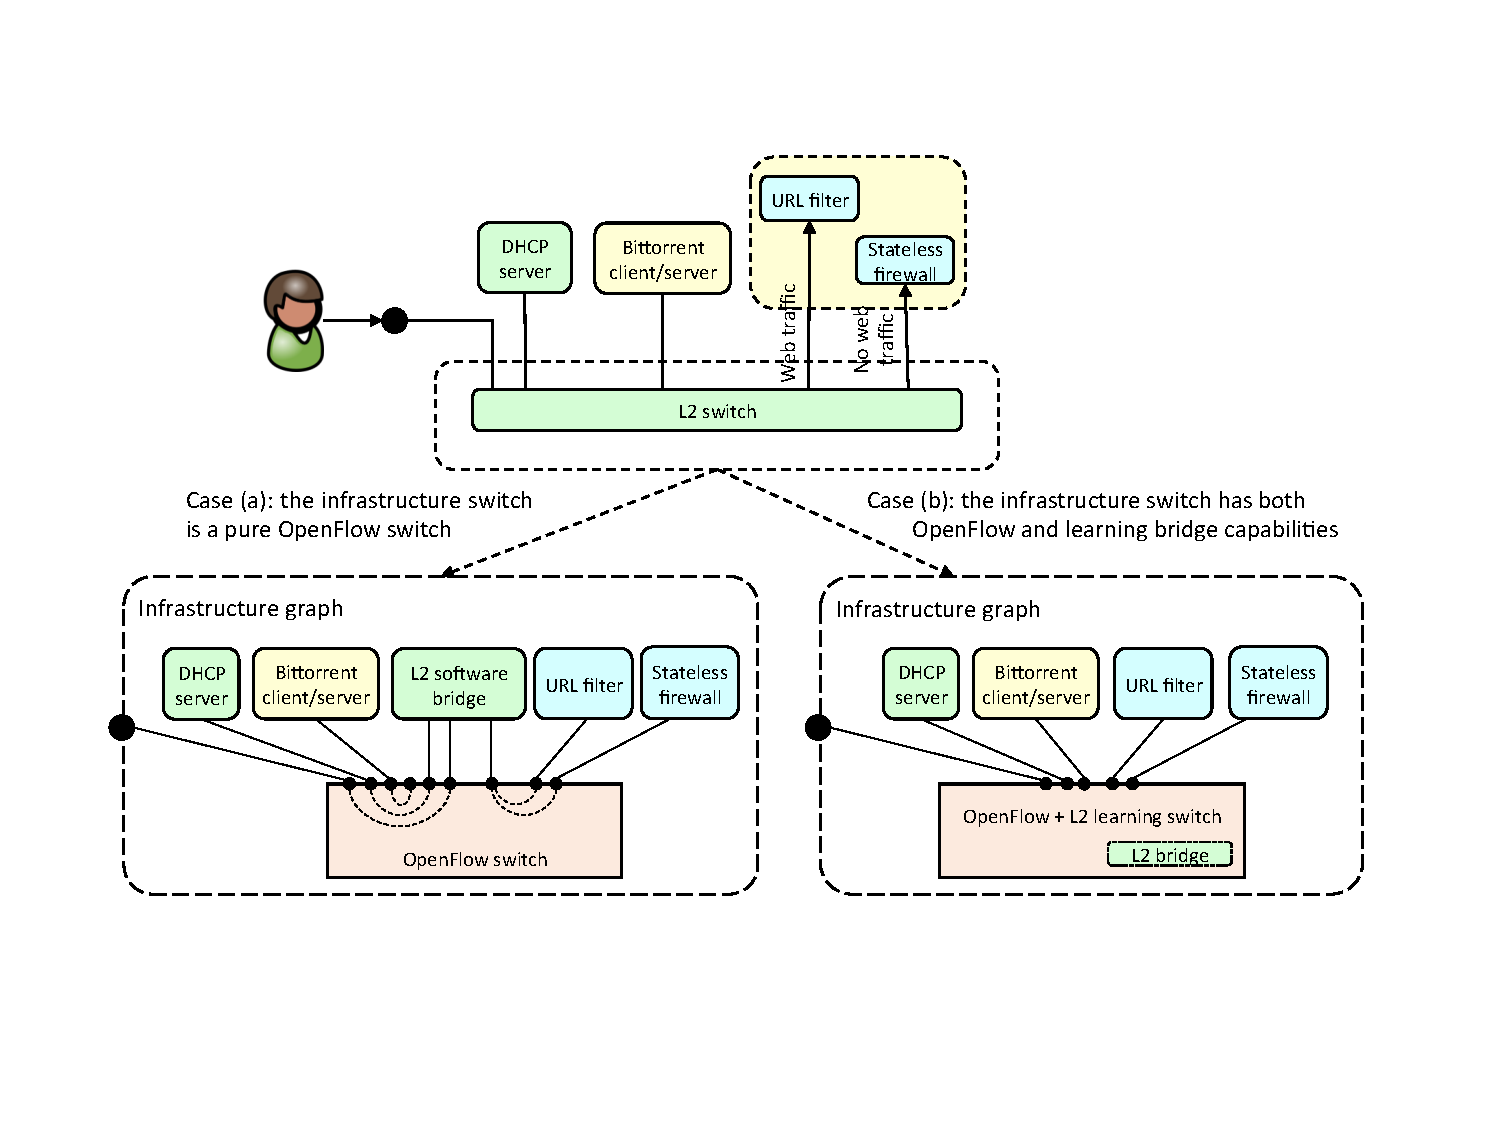
\includegraphics[clip= true, width= 0.8\columnwidth, trim= 0in 1.5in 0in 0in]{images/NF-FG_reconciliation.pdf}
	\caption{Part of the reconciliation process.}
	\label{fig:infrastructure_graph}
\end{figure}

Second, the flow rules defining the links of the FG, i.e., the connections among the VNFs, are properly translated according to the technology used by the physical node to implement the graph.
For example, if the physical node interconnects the VNFs through an Openflow vSwitch, each flow rule is converted in a number of Openflow \texttt{flowmod} messages.
However, other implementations of the infrastructure layer could implement these connections through other technologies, such as GRE tunnels or VLAN tags.

Similarly, each VNF is converted in the commands required to retrieve the image and start it up; also in this case, these commands depend on the technology implementing the VNFs (e.g., virtual machine, Docker containers, etc.).







\section{VNF template}
\label{chap:VNFdescriptor}
\label{sec:template}
As introduced above, each network function is associated with a template, which describes the VNF itself both in terms of infrastructure and in terms of configuration; an example of such a template is provided in Listing \ref{lst:NF-FG_templete}.

\lstinputlisting[label=lst:NF-FG_templete, language=python, caption={NF-FG - VNF template.}]{code/template2.txt}

As evident from listing example, the template contains some information related to the hardware required by the VNF, namely the amount of memory and CPU, as well as the architecture of the physical machine that can execute it and the requirements of disk in terms of swap, root file system and ephemeral file system size. Moreover, the boolean element \texttt{expandable} indicates if the VNF consists of a single image, or if it is actually a subgraph composed of several VNFs connected together. In the former case, the \texttt{uri} element refers to the image of the VNF, while in the latter it refers to a graph description, which must replace the original VNF in the forwarding graph. In case of non-expandable VNF, the template also specifies the type of the image; for instance, the firewall described in Listing \ref{lst:NF-FG_templete} is implemented as a single virtual machine.
Moreover, the template provides a description of the ports of the VNF, each one associated with several parameters. In particular, the label specifies the purpose of that port, and it is useful in the definition of the SG, since it helps to properly connect the VNF with the other components of the service (e.g., the external port of the firewall should be connected towards the Internet, while the internal ones should be connected towards the users). The label could assume any value, and it is meaningful only in the context of the VNF. The parameter \texttt{ipv4-config}, instead, indicates if the port cannot be associated with an IPv4 address (none), or if it can be statically (static) or dynamically (DHCP) configured, the same applies to \texttt{ipv6-config}. The field position specifies both the number of the ports of a certain type and the internal index of the interfaces. The number of ports is given by the difference between the second and the first  number of the range more one (e.g. \texttt{"position": "1-2"} means there are 2 ports of that label), it is also possible to insert \texttt{N} as value of last number of the range to indicate a variable number of interfaces available on VNF. For instance, the VNF of the example has one control port (or no one), one external port, and at least one internal port (in fact, it has a variable number of internal ports, which can be selected during the definition of the SG).  Position specifies also, along to the field name, the effectively name of the internal interface of VNF. In particular, the first number in the range of field position acts as an offset for the id used to reference a port in FG. For example, if the FG there is a port with id equals to "internal:2" (hence we have at least three ports labeled as internal), the name of the internal interface of the VNF is "eth4", because the value position for ports labeled as internal is "2-N" and the value of field name is "eth".
Obviously, as explained above, a VNF must have not more of one port type with a name with variable number interface.

\begin{comment}
\fabio{root-file-system-size c'e' il sistema e deve essere grande almeno quanto l'immagine
ephemeral non ho capito un cazzo, l'unica cosa certa e' che alla morte della macchina scompare}
\end{comment}












\begin{comment}

\section{Infrastructure graph}
\label{sec:ig}

The FG described so far, in order to be deployed on the physical infrastructure, must be mapped on the resources (both physical and software) available on the node on which the service is going to be instantiated. This new representation of the service is called infrastructure graph (IG), and it is obtained through the so called reconciliation process. More in detail, the reconciliation includes the transformations described in the following.
First, the graph endpoints are converted into: (i) physical ports of the server in which the graph is going to be instantiated, or (ii) tunnel endpoints (e.g., GRE) in order to connect two pieces of the same service but deployed on different physical nodes. Second, some of the VNFs in the FG could be mapped on resources available on the node, instead of being implemented as a specific image. For example, as depicted in the left of Figure \ref{fig:NF-FG_reconciliation}, if the node exploits a pure Openflow switch (e.g., xDPd \cite{xdpdwebsite}) to interconnect the VNFs of the graph, all the VNFs specified in the FG will be implemented through the proper images. Otherwise, if the vSwitch also implements the MAC learning algorithm (hence, it is not a pure Openflow switch, such as Open vSwitch \cite{ovswebsite}, the switch VNFs in the FG are removed, since their functionalities are already implemented by the vSwitch itself.
\fabiodubbio{forse cancellare questa parte non e' una cattiva idea}
Third, the flow rules shown in Figure 4, which defines the links of the FG, are properly translated according to the technology used to by the physical node to implement the graph. For example, as described later in the paper, when the physical node implements the graph through an Openflow switch such as xDPd or Open vSwitch, each flow rule is converted in a number of Openflow flowmod messages.

\begin{figure}[h]
	\centering
	% left bottom right top
	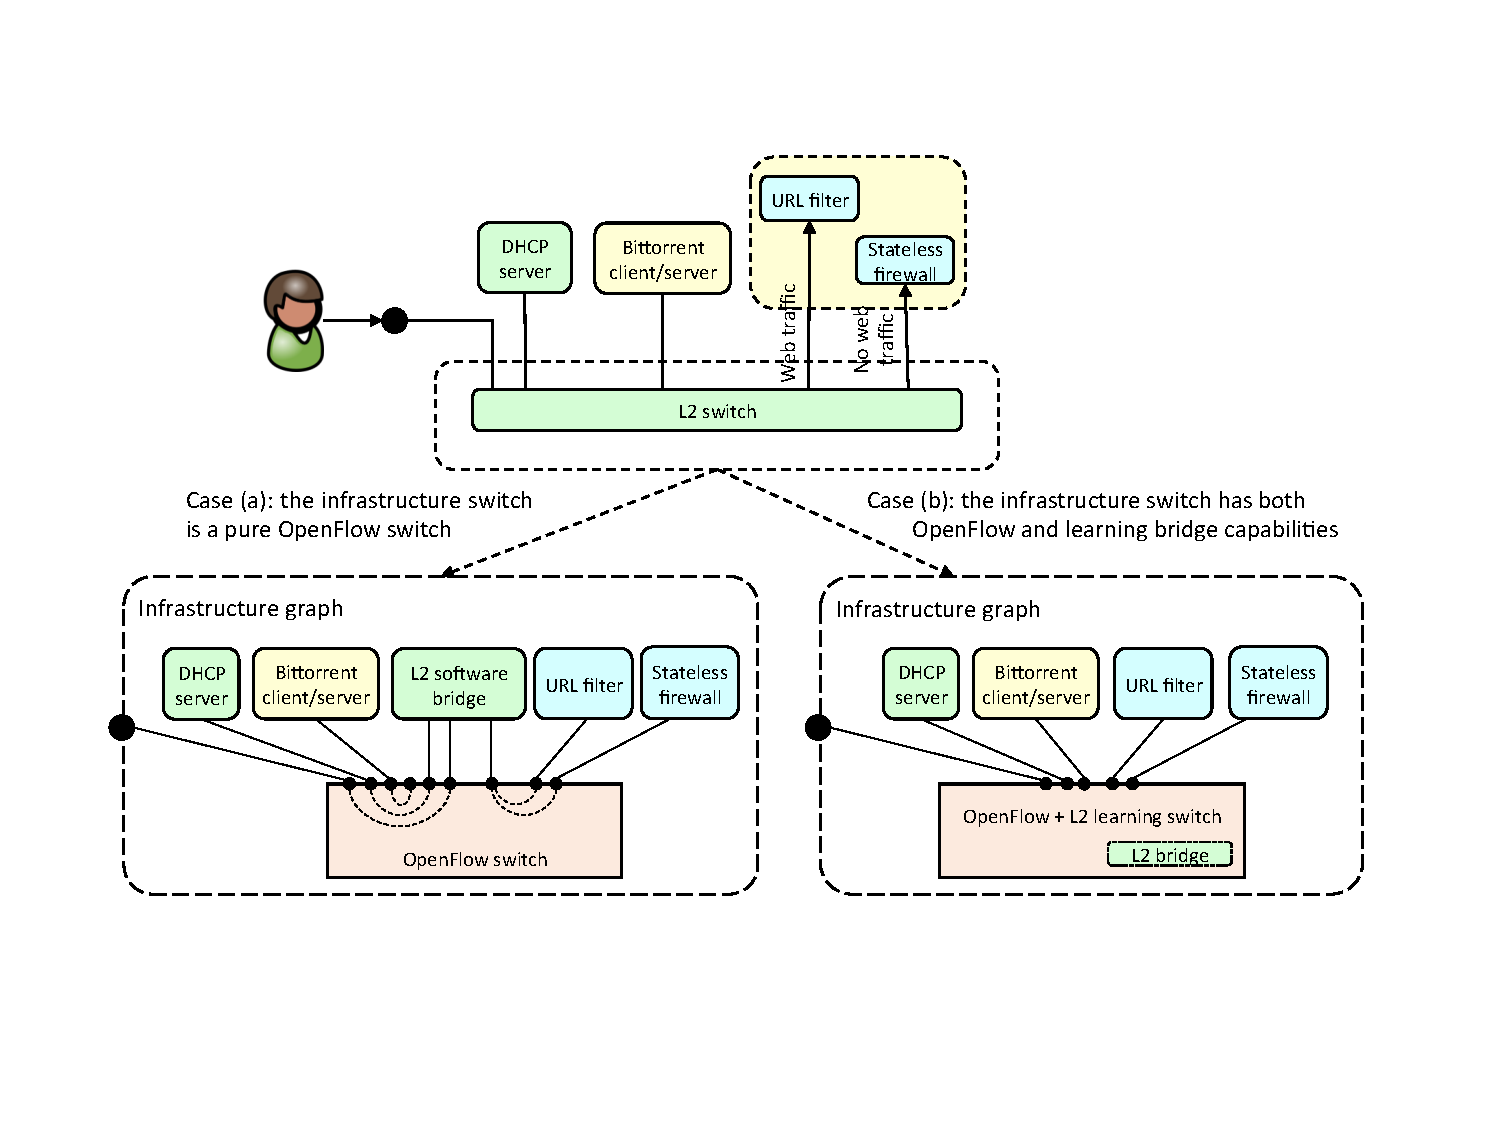
\includegraphics[clip= true, width= \columnwidth, trim= 0cm 1.8cm 0.2cm 2.0cm]{images/NF-FG_reconciliation.pdf}
	\caption{NF-FG - Reconciliation}
	\label{fig:NF-FG_reconciliation}
\end{figure}
\end{comment}
